

\section{Complexity of NCDN problem}
\label{sec:npcreduction}


\begin{figure*}
\centering
\vspace{-0.2in}
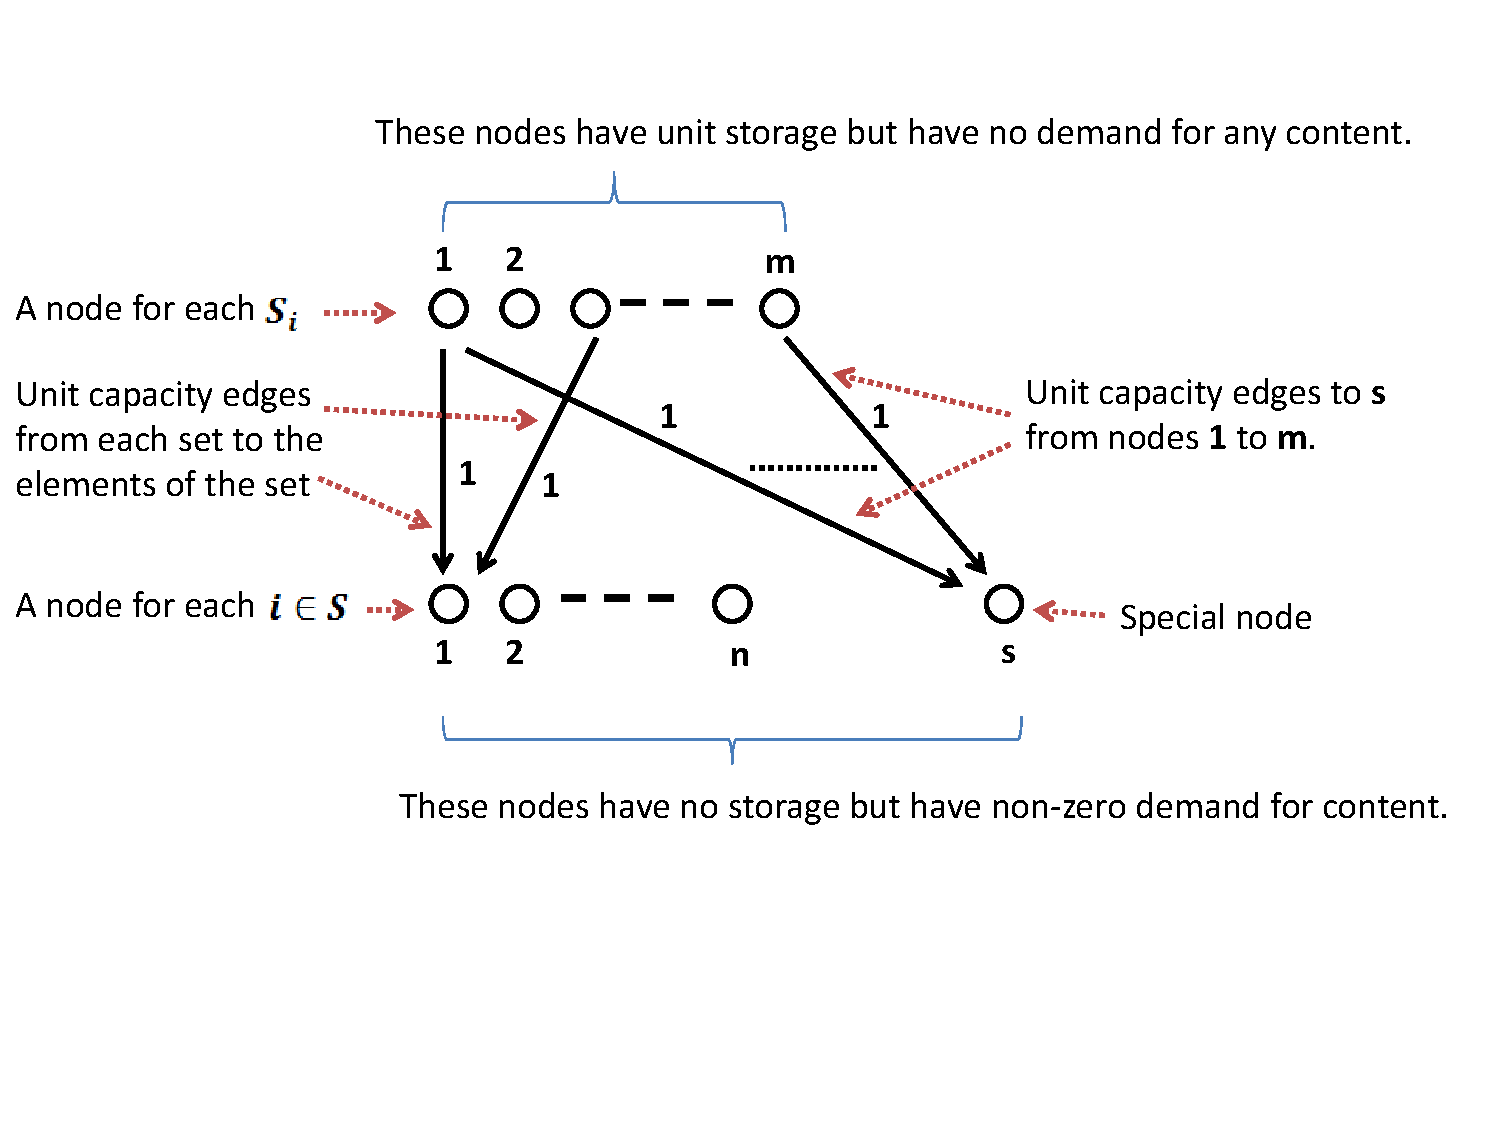
\includegraphics[scale=0.45]{graphSet1/setcover-reduction-diagram.pdf}
\vspace{-1in}
\caption{Reduction from \setcover\ to \optloc}
\label{fig:setcover}
\end{figure*}

%We show that the NCDN-problem is NP-Complete and is inapproximable to within an exponential factor.  

\optloc\ is the decision version of the NCDN problem described in $\S$\ref{sec:optimize}.  \optloc\ asks if the MLU of the network can be $\alpha$ while satisfying the constraints of the problem.

{{\sc Theorem 1}} {\em \optloc\ is NP-Complete even in the special case where all objects have unit size, all demands have unit value, and link and storage capacities have binary values.}



{\em Proof:} We show  a reduction from the well known \setcover\ problem.  We first define the \setcover\ problem that we will reduce to \optloc. 

{\bf \setcover}: Let $S = \{1, 2, ..., n\}$ be a set of $n$ elements. Let $X = \{S_1, ..., S_m\}$ where $S_i \subseteq\ S, 1 \leq i \leq m$. Let $k$ be an integer. \setcover\ asks if there exists  $Y = \{ Y_1, ..., Y_k\}$, where $Y_k \in X$ and $Y_1 \cup ... \cup Y_k = S$. Set $Y$ is called a set cover of size $k$.

%set cover\footnote{Arun: what if I don't know what a set cover is?}  of size $k$?


The reduction from \setcover\ to \optloc\ is described using the network in Figure \ref{fig:setcover}. Set $V_1 = \{1, ..., m\}$  refers to nodes in the top row. Each node $i \in V_1$ maps to the set $S_i \subset S$. Set $V_2 = \{1, ..., n\}$ refers to nodes in the bottom row excluding node $s$. Each node $i \in V_2$ maps to  element $i \in S$. Node $s$ is called a special node. 


Directed links $(i, j)$ exist from all nodes $i \in V_1$ to all nodes $j \in V_2$. The capacity of $(i,j)$ is 1 unit if $i \in S_j$, otherwise capacity is zero. Node $s$ has incoming links $(i, s)$ from all nodes  $i \in V_1$ such that  the capacity of all incoming links is 1 unit.

All nodes in the top row $V_1$ have unit storage whereas nodes in the bottom row $V_2\cup \{s\}$ have zero storage.

The set of objects is $\{o, 1, 2, ..., (m-k)\}$ and all objects have unit size. Object $o$ is a special object that has unit demand at nodes in set $V_2 = \{1, ..., n\}$ and zero demand at all other nodes. Objects $1$, $2$, .. $(m-k)$ have unit demand at special node $s$ and zero demand at all other nodes.

% The rest of the demands are zero. 

{\sc Claim:} There is a set cover of size $k$ if and only if the above network can achieve MLU $\leq$ 1.

\emph{If there is a set cover of size $k$, then the network can achieve MLU of 1.} Store the special object $o$ at the $k$ set cover locations in the top row and satisfy demand for $o$ at nodes  $V_2 = \{1, ..., n\}$ in the bottom row from these locations with MLU = 1. The remaining $(m-k)$ nodes in the top can be used for objects $\{1, 2, ..., (m-k)\}$ to satisfy the demand at special node $s$ with MLU of 1.

\emph{If there is no set cover of size k, then the network must have a MLU $>$ 1.} Objects must be placed in some $(m-k)$ nodes in the node $V_1 = \{1, ..., m\}$ in the top row to satisfy the demand for special node $s$. Thus, at most $k$ nodes are available for placing special object $o$. Since there is no set cover of size $k$,  some bottom node $i \in V_2$  must satisfy its demand for special object $o$ using an edge whose capacity is zero  resulting in MLU = $\infty$ on that edge.
%$\frac{1/k}{1/(m(\alpha\ + 1))} = \frac{(\alpha + 1)m}{k} \geq \alpha + 1 > 1$. 

It is easy to show that \optloc\ $\in$ NP. Hence, \optloc\ is NP-Complete.

\vspace{0.2in}

{{\sc Theorem 2}} {\em  \optloc\ is inapproximable within a factor $\beta$  for any $\beta > 1$ unless P = NP.}

\vspace{0.1in}

The proof of {\sc Theorem 1} shows that if there is a set cover of size $k$, MLU = 1 and MLU $= \infty$ otherwise. Thus, if we find a solution for which MLU is finite, it implies that MLU = 1, which immediately gives a solution to the corresponding \setcover\ instance.

Lets assume a  $\beta$-approximation ($\beta > 1$) exists for \optloc. Then, we can solve \setcover\ in polynomial time by mapping \setcover\ instance to \optloc\  instance, and checking if MLU $\leq \beta$ (which implies MLU = 1).  As \setcover\ $\in$ NP-Complete, therefore, no $\beta-$approximation for \optloc\ exists unless P = NP.

\section{Joint optimization of \\
transit traffic matrix \\
and content matrix}
\label{sec:ttmcm}

We present here a modification to the MIP in $\S$\ref{sec:linearprograms} to jointly optimize routing for an ISP transit traffic matrix (TTM) and a content matrix. Let $D$ be a TTM  and  $D_{ij}$ denote the traffic from PoP $i$ to PoP $j$. We modify only the constraints (3) and (4) in the earlier MIP as follows:

\begin{eqnarray}
\sum_{k \in K} t_{ijk}  + D_{ij}  &=& f_{ij} ,  \ \forall j \in V-X, i \in V
\end{eqnarray}
\begin{eqnarray}
\sum_{k \in K} t_{ijk} + \sum_{k \in K} \delta_{ij}  t_{iok}   + D_{ij} &=& f_{ij} ,  \ \forall j \in X, i \in V
\end{eqnarray}



\section{Limiting content placement\\ update traffic}
\label{sec:placementupdate}
In this section, we describe our extension to the MIP presented in $\S$\ref{sec:linearprograms} which allows us to limit the MLU due to traffic from updating the content placement. To this end, we add constraints to the MIP to ensure that the MLU due to the placement update traffic is less than a constant $\beta$. In our experiment, we dynamically update the value of $\beta$ to be two/third of the MLU within the past 24 hours of the experiment. 

We follow the same notation as in $\S$\ref{sec:linearprograms}. The binary variable $x_{ik}$ denotes if the content $k \in K$ is stored at node $i \in V$, $S_k$  denotes the size of the content.  
To describe the constraint, we  define the following parameters :  $T$ denotes the duration over which traffic due to placement update will be spread out.   $X_{jk}$ denotes whether content $k \in K$ is stored at node $j \in V$ currently. The current routing in the network is $r_{ije}$,  the fraction of traffic  from node $j$ to node $i$ crossing link $e$.  In addition we define a function  $\gamma(i, j, k)$.  $\gamma(i, j, k) = 1$  if $X_{jk} = 1$ and node $j$ is the closest node in terms of hop count from node $i$ which has stored a copy of content $k$, otherwise.  Both $r_{ije}$ and $\gamma(i, j, k)$ depend on current routing and placement in the network and hence are known constants.
We assume that the transfer of content of size $S_k$ happens at a constant bit rate of $S_k/T$. In terms of these variables we can define the total traffic  $u_e $ on any link $e \in E$ during the placement update period. 

\begin{eqnarray}
u_e = \sum_{i \in V}  \sum_{j \in V}  \sum_{k \in K}  \gamma(i, j, k) r_{ije}  x_{jk} S_k / T \quad \forall e \in E
\end{eqnarray}

Finally, in order to limit the maximum utilization of any link $e \in E$, we add the following constraint, 

\begin{eqnarray}
 u_e /C_e < \beta \quad \forall e \in E
\end{eqnarray}




%%%%%%%%%%%% PROOF FROM PARTITION%%%%%%%%%%%%

\eat
{
\section{\optloc\ is NP-Complete}
\label{sec:npcreduction}



\optloc\ is the decision version of the NCDN problem described in $\S$\ref{sec:optimize}.  \optloc\ asks if the MLU of the network can be $\alpha$ while satisfying the constraints of the problem.

We reduce Partition to \optloc. Partition asks whether a given set A of positive integers can be partitioned into  subsets A1 and A2 such that the sum of the numbers in A1 equals the sum of the numbers in A2. For our reduction, we define an instance of  \optloc\ in terms of  the inputs to Partition. See Table \ref{table:paramtable} for a list of input variables to \optloc.
%the value for each input  variable for \optloc\ (see Table \ref{table:paramtable}) in terms of the inputs to Partition. 


%\noindent{\textbf{Network model:}}  The network is a graph $G(V, E)$ and  serves a set of traffic demands $F=\{f_1,f_2, ...\}$ at sink nodes $N = \{n_1, n_2, ...\}$. A set of source nodes $M =\{m_1, m_2, ...\}$ serve the demands to all the sink nodes.



%The MLU of the network for a set of sources can be calculated by solving the MIP  in $\S$\ref{sec:optimize}. 


%For a network $G(V, E)$ and a set of demands $F=\{f_1,f_2, ..., f_m\}$ at sink nodes $N = \{n_1, n_2, ..., n_m\}$, select source nodes $S =\{s_1, s_2, ..., s_k\}$ such that the optimal MLU for this network calculated using linear program is minimized.

%We define the problem \minsubsetsum\ which we show to be NP-hard by reduction from the \subsetsum\ problem.

\vsp

\noindent\emph{Nodes:} $V = \{1, 2, 3\}$. 

\vsp

\noindent\emph{Edges:}  $E =  \{ (2, 1) , (3, 1)\}$. Notation (x, y) means a directed link with  source = x,  destination = y.

\vsp

\noindent\emph{Nodes connected to origin:}  $X = \phi$ (null set).

\vsp

\noindent\emph{Disk space:}  $D_1 = 0, D_2 =  D_3 = (\sum_{a \in A} a)/2$.

\vsp

\noindent\emph{Link capacity:}  $C_{(1, 2)} = C_{(2, 3)} = \sum_{a \in A} a$.

\vsp

\noindent\emph{Content set:}  $K = \{1, 2, ..., |A|\} $. There is a bijective mapping from the content set K to the integer set A.

\vsp

\noindent\emph{File size:}  $S_{i} = a_i$  such that $ a_i \in A$.

\vsp

\noindent\emph{Content demand at nodes:}  $T_{1i} = a_i, T_{2i} = T_{3i} = 0,  \forall i \in K$.

%$T_{ik} = \delta$ $ \forall i \in V2, k \in  K - \{1\}$, where $0 < \delta << 1$ and $\delta <<  \textit{min} ( c_e ) \forall e \in E$. $T_{ik} = 0$ $ \forall i \in V1, \forall k \in K$.

This instance of \optloc\ asks if the MLU can be $\alpha = 1/2$ while satisfying the constraints of the problem. 

We first show that solution to Partition also gives a solution to \optloc. Let $A1 = \{a1_1, ... \}$ and  $A2 = \{a2_1, ... \}$ be the two partitions the sum of whose elements are equal.  We store the content corresponding to the integers in set A1 (set A2) at node  2 (node 3). Size of the content stored at node 2 = $\sum_{a1_i \in A1} a1_i =  (\sum_{a \in A} a)/2$, which satisfies the disk space constraints at node 2  (Similar argument works for node 3). Traffic on link (2, 1) = $\sum_{a1_i \in A1} a1_i =  (\sum_{a \in A} a)/2$. So, utilization of link (2, 1) is 1/2.  Similarly, utilization of link (3, 1) can be shown to be 1/2. Hence, the MLU is 1/2.


Next, we show that a solution to \optloc\ can be mapped to a solution to Partition. For a feasible solution to \optloc\ problem, let $A1 = \{a1_1, ... \}$ and  $A2 = \{a2_1, ... \}$ be the sets of sizes of content stored at node 2 and node 3 respectively. We put the integers corresponding to the content stored at node 2 (node 3) in the first (second) partition. Clearly, sum of integers in the two partitions are equal : $\sum_{a1_i \in A1} a1_i   = \sum_{a2_i \in A2} a2_i = (\sum_{a \in A} a)/2$.

It is easy to show that \optloc\ $\in$ NP. Partition is NP-Complete, therefore, \optloc\ is  NP-Complete. 

}


\eat{

\section{Complexity of NCDN problem}
\label{sec:npcreduction}


\begin{figure*}
\centering
\vspace{-0.2in}
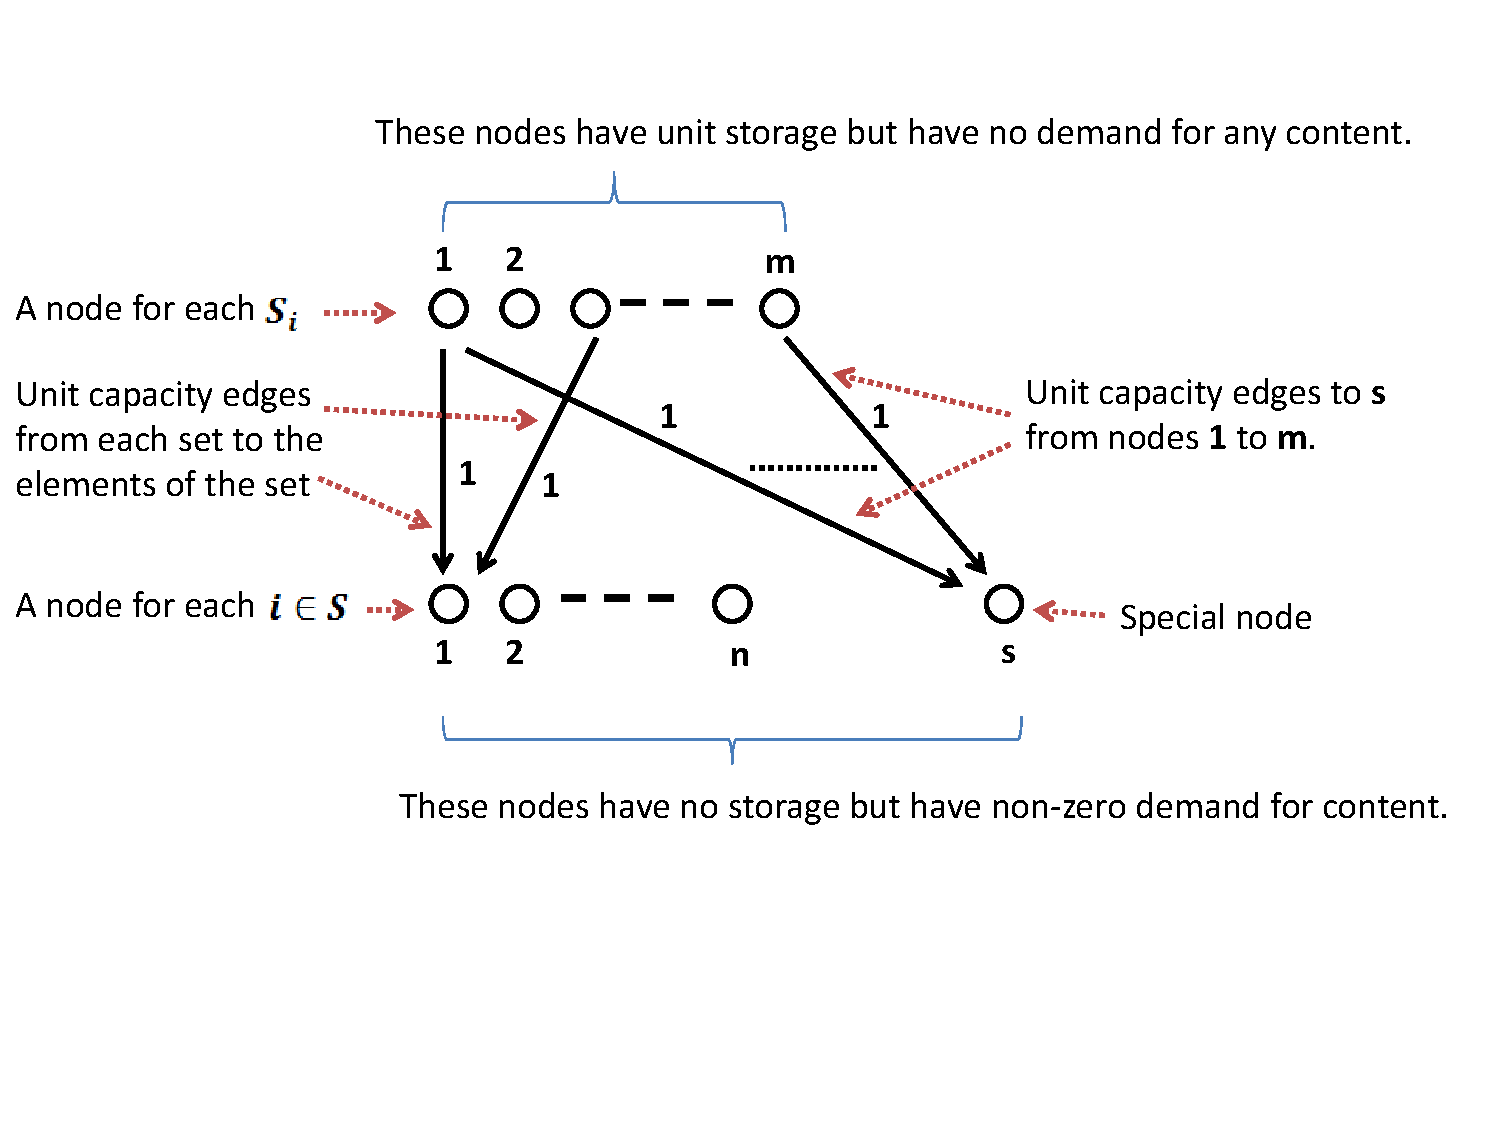
\includegraphics[scale=0.45]{graphSet1/setcover-reduction-diagram.pdf}
\vspace{-1in}
\caption{Reduction from \setcover\ to \optloc}
\label{fig:setcover}
\end{figure*}

%We show that the NCDN-problem is NP-Complete and is inapproximable to within an exponential factor.  

\optloc\ is the decision version of the NCDN problem described in $\S$\ref{sec:optimize}.  \optloc\ asks if the MLU of the network can be $\alpha$ while satisfying the constraints of the problem.

{{\sc Theorem 1}} {\em \optloc\ is NP-Complete even in the special case where all objects have unit size, and all demands have unit value.}



{\em Proof:} We show  a reduction from the well known \setcover\ problem.  We first define the \setcover\ problem that we will reduce to \optloc. 

{\bf \setcover}: Let $S = \{1, 2, ..., n\}$ be a set of $n$ elements. Let $S_i \subseteq\ S, 1 \leq i \leq m$ be m subsets of set $S$. Let $k$ be an integer. \setcover\ asks if  there is a set cover\footnote{Arun: what if I don't know what a set cover is?}  of size $k$?


The reduction from \setcover\ to \optloc\ is described using the network in Figure \ref{fig:setcover}. Set\footnote{Arun: change V1 to $V_1$.}  $V1 = \{1, ..., n\}$  refers to nodes in the top row. Each node $i \in V1$ maps to element $i \in S$. Set $V2 = \{1, ..., m\}$ refers to nodes in the bottom row excluding node $s$. Each node $i \in V2$ maps to the set $S_i \subset S$. Node $s$ is called a special node. 


Directed links $(i, j)$ exist from all nodes $i \in V1$ to all nodes $j \in V2$. The capacity of $(i,j)$ is 1 unit if $i \in S_j$, otherwise capacity is $\frac{1}{n(\alpha + 1)}$, where $\alpha > 0$ is a very large value. Node $s$ has incoming links $(i, s)$ from all nodes  $i \in V1$ such that  the capacity of all incoming links is 1 unit.

All nodes in the top row $V1$ have unit storage whereas nodes in the bottom row $V2\cup \{s\}$ have zero storage.

The set of objects is $\{o, 1, 2, ..., (n-k)\}$ and all objects have unit size. Object $o$ is a special object that has unit demand at nodes in set $V2 = \{1, ..., m\}$ and zero demand at all other nodes. Objects $1$, $2$, .. $(n-k)$ have unit demand at special node $s$ and zero demand at all other nodes. 

% The rest of the demands are zero. 

{\sc Claim:} There is a set cover of size $k$ if and only if the above network can achieve MLU $\leq$ 1.

\emph{If there is a set cover of size $k$, then the network can achieve MLU of 1.} Store the special object $o$ at the $k$ set cover locations and satisfy demand for $o$ at nodes  $V2 = \{1, ..., m\}$ from these locations with MLU = 1. The remaining $(n-k)$ nodes in the top can be used for objects $\{1, 2, ..., (n-k)\}$ to satisfy the demand at special node $s$ with MLU of 1.

\emph{If there is no set cover of size k, then the network must have a MLU $>$ 1.} Objects must be placed in some $(n-k)$ nodes in set $V1 = \{1, ..., n\}$ to satisfy the demand for special node $s$. Thus, at most $k$ nodes are available for placing special object $o$. Since there is no set cover of size $k$,  some bottom node $i \in V2$  must satisfy its demand for special object $o$ using edges whose capacity is $\frac{1}{n(\alpha + 1)}$. Therefore, at least one of these edges must route $\geq 1/k$ unit of demand causing an MLU of 
$\frac{1/k}{1/(n(\alpha\ + 1))} = \frac{(\alpha + 1)n}{k} \geq \alpha + 1 > 1$. 

It is easy to show that \optloc\ $\in$ NP. Hence, \optloc\ is NP-Complete.
\vspace{0.3in}

{{\sc Theorem 2}} {\em  \optloc\ is inapproximable within a $2^{O(I)}$ factor unless P = NP, where $I$ is the input size of the problem.}

\vspace{0.1in}
The proof of {\sc Theorem 1} shows that when there is a set cover of size $k$, MLU = 1 and MLU $\geq \alpha +1$ otherwise. If there is an $\alpha$-approximation for \optloc\ then we can solve \setcover\ by reducing the set-cover instance to an NCDN instance by mapping the $\alpha-$approxmation and checking if MLU$ \leq \alpha $ or not. Thus, no $\alpha-$approximation for \optloc\ is possible unless P = NP. 


How large can $\alpha$ be? The only restriction is that the reduction be polynomial in $(n + m)$. With this restriction, we can represent a value $\alpha = 2^{{\textit{Poly}}(n+m)} =2^{O(I)}$, where $I$ is the input size of the \optloc\ problem. Thus, no $2^{O(I)}$-approximation for \optloc\ is possible, where $I$ is the input size of the \optloc\ problem unless P = NP. 
}





%%Thus, \optloc\ returns Yes, only if 
%
%% (\sum_{a \in A} a)/2 
%
%%We show that the answer to Partition problem is Yes if and only if the answer of the corresponding \optloc\ problem is also Yes. 
%
%
%%First we prove that the optimal allocation will have content $k_1$ at $r$ locations and content $k_2, k_3, ..., k_{p - r +1}$ at 1 location each. 
%
%
%
%
%\eat
%{
%
%
%\section{\optloc\ is NP-Complete}
%\label{sec:npcreduction}
%
%
%
%We first reduce \subsetsum\ to \minsubsetsum\ and next reduce \minsubsetsum\ to \optloc. 
%
%%\noindent{\textbf{Network model:}}  The network is a graph $G(V, E)$ and  serves a set of traffic demands $F=\{f_1,f_2, ...\}$ at sink nodes $N = \{n_1, n_2, ...\}$. A set of source nodes $M =\{m_1, m_2, ...\}$ serve the demands to all the sink nodes.
%
%\vsp
%{\bf{\optloc:}}  \optloc\ is the decision version of the NCDN problem described in $\S$\ref{sec:optimize}.  \optloc\ asks if the MLU of the network can be $\alpha$ while satisfying the constraints of the problem.
%
%%The MLU of the network for a set of sources can be calculated by solving the MIP  in $\S$\ref{sec:optimize}. 
%
%
%%For a network $G(V, E)$ and a set of demands $F=\{f_1,f_2, ..., f_m\}$ at sink nodes $N = \{n_1, n_2, ..., n_m\}$, select source nodes $S =\{s_1, s_2, ..., s_k\}$ such that the optimal MLU for this network calculated using linear program is minimized.
%
%%We define the problem \minsubsetsum\ which we show to be NP-hard by reduction from the \subsetsum\ problem.
%
%\vsp
%
%\textbf{\minsubsetsum:} Let $D = \{D_1, D_2, ..., D_q\}$, where $D_i = (d_{i1}, d_{i2}, ..., d_{ip})$ be an  integer array of length $p$. Let $a$ be an two integer. \minsubsetsum\ problem asks if there are $r$ indices $(0 < r \leq p)$ $j_1, j_2, ..., j_r$ such that $ \textit{min}(x_1, x_2, ... , x_q) = a$, where $x_i = d_{ij_1} + d_{ij_2} + ... + d_{ij_r}$.
%%$C_i$ each of length $p$.
%
%\vsp
%\textbf{Reduction from \subsetsum\ to \minsubsetsum:} 
%Let $B = \{ b_1, b_2, b_3, ..., b_p\}$ be a set of integers and $a$ be a given integer. \subsetsum\ problem asks if there is a subset of $B$ the sum of whose elements is $a$. 
%
%We can reduce this to \minsubsetsum\ as follows: We define $C = \{B_1\}$, where $B_1 =  \{b_1, ..., b_p\}$.  We ask the following \minsubsetsum\ problem for a given \subsetsum\ problem: are there $r$ indices $(0 < r \leq p)$ $j_1, j_2, ..., j_r$ such that $\textit{min} (x1) = a$, where $ x_1 =  B_1[j_1] + B_1[j_2]  + ... + B_1[j_r]$.  If \minsubsetsum\ returns the answer Yes, then the answer to the \subsetsum\ problem is also Yes. Otherwise, the answer to \subsetsum\ is No. Thus, we have shown a polynomial time  reduction from \subsetsum\ to \minsubsetsum.
%
%\vsp
%\textbf{Reduction from \minsubsetsum\ to \optloc:}
%We transform a  \minsubsetsum\ problem to an instance of \optloc\ problem. For this purpose, we describe the value for each variable in Table \ref{table:paramtable} in terms of the inputs to the problem \minsubsetsum. 
%\begin{itemize}
%\item $V = \{1, 2, ..., p + q\}$. We define two subsets of $V$,  $V1 = \{1, ..., p\}$, $V2 = \{p+1, ..., p + q\}$.
%\item $E =  \{ (i, j) : \forall i \in V1, \forall j \in V2\}$.
%\item $X = \phi$, implying there is no origin node.
%\item $D_i = 1 \forall i \in V1, D_i = 0 \forall i \in V2$.
%\item $C_e = C_{ij} = d_{i(j - p)}, \forall i \in V1, \forall j \in V2$.
%\item $K = \{k_1\} $
%\item $S_{k_1} = 1$
%\item $T_{i1} = 1, \forall i \in V2$. 
%\end{itemize}
%%$T_{ik} = \delta$ $ \forall i \in V2, k \in  K - \{1\}$, where $0 < \delta << 1$ and $\delta <<  \textit{min} ( c_e ) \forall e \in E$. $T_{ik} = 0$ $ \forall i \in V1, \forall k \in K$.
%
%
%\optloc\ decision problem corresponding to  an instance of \minsubsetsum\ problem asks if the MLU of the network can be $1/a$ while satisfying the constraints of the problem.  We show that the answer to \minsubsetsum\ problem is Yes if and only if the answer of the corresponding \optloc\ problem is also Yes. 
%
%%First we prove that the optimal allocation will have content $k_1$ at $r$ locations and content $k_2, k_3, ..., k_{p - r +1}$ at 1 location each. 
%
%Let us assume that content $k_1$ is stored at $r$ locations $X =\{ x_{1}, x_{2}, ... x_{r} \}$ where each $x_{i} \in V1$.  Note that content $k1$ is of size 1 and storage at any node $i \in V1$ is 1. Therefore, at most one content can be stored at each node $i \in V2$. As there is exactly one path between any node $i \in V1$ and  $j \in V2$, which is the link $(i, j)$, all traffic from node $i$ to node $j$ goes through link $(i, j)$. Further, there is only one content at each node $i$, therefore, link $(i, j)$ carries the traffic only for the content stored at node $i$.
%
%\eat
%{
%Let us assume that content $k_1$ is stored at $r$ locations $X =\{ x_{1}, x_{2}, ... x_{r} \}$ where each $x_{i} \in V1$. Content $k_2, k_3, ..., k_{p - r +1}$ is stored at $Y =\{  y_2, y_3 ..., y_{p - r + 1}\}$ respectively, where each $y_i \in V1$. Note that all content is of size 1 and storage at any node $i \in V1$ is 1. Therefore, at most one content can be stored at each node $i \in V2$. As there is exactly one path between any node $i \in V1$ and  $j \in V2$, which is the link $(i, j)$, all traffic from node $i$ to node $j$ goes through link $(i, j)$. Further, there is only one content at each node $i$, therefore, link $(i, j)$ carries the traffic only for the content stored at node $i$.
%}
%%Moreover, each link $(i, j) i \in V1, j \in V2$ carries the traffic only for content stored at node $i$ to node $j$.
%
%
%Let $L = \{l_j :   l_j = \sum_{x_i}  d_{x_i(j - p)}, \forall j \in V2, \forall x_i \in X\}$. We claim that $\textit{MLU} = \frac{1}{\textit{min} (l_1, l_2, ... )}$.  Consider node $j \in V2$. $l_j$ is the total capacity of links from nodes where content $k_1$ is stored. The  demand for content $k_1$ at node $j \in V2$ is split across links $(i, j), i \in X, j \in V2$. To minimize the MLU, the traffic on each link $(i, j)  i \in X, j \in V2 $ is assigned proportional to its capacity. Therefore, utilization of link $(i, j)  = 1/l_j  i \in X, j \in V2$. Thus, the MLU over all links $(i, j),  i \in X, j \in V2 $ is $\frac{1}{\textit{min} (l_1, l_2, ... )}$.  Next, we show that  utilization of links $(i, j) i \in Y, j \in V2$ is smaller than $\frac{1}{\textit{min} (l_1, l_2, ... )}$, which proves our claim that $\textit{MLU} = \frac{1}{\textit{min} (l_1, l_2, ... )}$ in this case.
%
%
%Node $y_i$ stores content $k_{i}$. Also, $y_i$ is the only node where this content is stored. Therefore, the traffic on link $(y_i, j), j \in V2$  is $\delta$. As the capacity of link $(y_i, j)$ is $d_{x_{i}(j - p)}$, therefore the utilization of link $(y_i, j)$ is $\delta/d_{y_i(j - p)}$. 
%\[\frac{\delta}{d_{y_i(j - p)}} \leq \frac{\delta}{d\_min} << \frac{1}{S_j}  \leq \frac{1}{\textit{min} (l_1, l_2, ... )}\]
%
%Thus, we have shown that $\textit{MLU} = \frac{1}{\textit{min} (l_1, l_2, ... )}$.
%
%Next, we show that if $k1$ is stored at less than $r$ locations, the MLU will be higher. Note that  $k1$ cannot be stored at more than $r$ locations because other $(p - r)$ content must be stored at least at one location. Let us assume  $a \in X$  is removed from $X$, then $L1 = \{l1_j :  l1_j = \sum_{x_i}  d_{i(j - p)}, \forall x_i \in X - \{a\} \forall j \in V2\}$. Clearly, $\textit{min} (l_1, l_2, ... ) > \textit{min} (l1_1, l1_2, ... )$. The empty storage at node $a$ can be filled by any content $K - \{k1\}$.  However, this will not increase the utilization of any link $(i, j)$ where node $i$ has stored any content $K - \{k1\}$ and $j \in V2$. Overall, the utilization increases if $k1$ is stored at less than $r$ locations. 
%
%We have assumed that content $k1$ is stored at any $r$ locations. Therefore, even if the locations were chosen so that the resulting MLU is $\alpha$.
%
%
%%Note that utilization of other links (i, j), where node $i$ has stored content $j$ will not decrease.
%
%
%If the answer to \optloc\ problem is Yes, then the answer to  \minsubsetsum\ is also Yes. If the answer to \optloc\ problem is No, then the answer to  \minsubsetsum\ is also No. 
%
%Thus, we have shown a polynomial time reduction from \minsubsetsum\ to \optloc.
%
%%Otherwise, the answer to \minsubsetsum\ is also No. 
%
%
%
%As \subsetsum\ is NP-Hard, \optloc\ is NP-Hard. It is easy to show that \optloc\ $\in$ NP. Thus, \optloc\ $\in$ NP-Complete.
%
%
%\section{\optloc\ is NP-Complete}
%\label{sec:npcreduction}
%
%
%We first reduce \subsetsum\ to \minsubsetsum\ and next reduce \minsubsetsum\ to \optloc. 
%
%\noindent{\textbf{Network model:}}  The network is a graph $G(V, E)$ and  serves a set of traffic demands $F=\{f_1,f_2, ...\}$ at sink nodes $N = \{n_1, n_2, ...\}$. A set of source nodes $M =\{m_1, m_2, ...\}$ serve the demands to all the sink nodes.
%
%\vsp
%\noindent{\bf{\optloc:}} The \optloc\ problem is to select $k$ source locations in the network that minimize the MLU. The decision version of this problem asks if there are $k$ source locations such that the $MLU$ of the network is $\alpha$. 
%
%%The MLU of the network for a set of sources can be calculated by solving the MIP  in $\S$\ref{sec:optimize}. 
%
%
%%For a network $G(V, E)$ and a set of demands $F=\{f_1,f_2, ..., f_m\}$ at sink nodes $N = \{n_1, n_2, ..., n_m\}$, select source nodes $S =\{s_1, s_2, ..., s_k\}$ such that the optimal MLU for this network calculated using linear program is minimized.
%
%%We define the problem \minsubsetsum\ which we show to be NP-hard by reduction from the \subsetsum\ problem.
%
%\vsp
%\noindent\textbf{\minsubsetsum:} Let $C_i = (c_{i1}, c_{i2}, ..., c_{ip})$ be an integer array of length $p$. Let $C = \{C_1, C_2, ..., C_q\}$ be a set of integer arrays $C_i$ each of length $p$. Let $a$ and $r (0 < r \leq p)$  be two integers. The \minsubsetsum\ problem asks if there are $r$ indices $j_1, j_2, ..., j_r$ such that $ \textit{min}(x_1, x_2, ... , x_q) = a$, where $x_i = c_{ij_1} + c_{ij_2} + ... + c_{ij_r}$.
%
%\vsp
%\noindent\textbf{Reduction from \subsetsum\ to \minsubsetsum:} \\
%Let $B = \{ b_1, b_2, b_3, ..., b_p\}$ be a set of integers and $a$ be a given integer. The \subsetsum\ problem asks if there is a subset of $B$ the sum of whose elements is $a$. 
%
%We can reduce this to \minsubsetsum\ as follows: We make a array $B_1 = \{b_1, b_2, ..., b_p\}$ of length $p$ with elements of $B$. We define $C = \{ B_1 \}$. Therefore, $q = 1$. 
%%For each $k \in \{1, 2, ..., p\}$, 
%We ask the following \minsubsetsum\ problem: are there $k$ indices $j_1, j_2, ..., j_k$ such that $\textit{min} (x_0) = a$, where $ x_0 = B_1[j_1] + B_1[j_2]  + ... + B_1[j_k]$. For any value of $k$, if \minsubsetsum\ returns the answer Yes, then the answer to the \subsetsum\ problem is also Yes. Otherwise, the answer to \subsetsum\ is No. Thus, we have shown a polynomial time (how?)  reduction from \subsetsum\ to \minsubsetsum.
%
%\vsp
%\noindent\textbf{Reduction from \minsubsetsum\ to \optloc:}\\ 
%We reduce the \minsubsetsum\ problem defined above to \optloc.  Since the capacity of links in the network is more than zero, we assume $c_{ij} > 0$. % rational
%
%Let $N = \{n_1, n_2, ..., n_p\}$, $M' = \{m_1, m_2, ..., m_p\}$, and $ G = N \cup M'$.
%
%
%
%
%The set of nodes $M'$ is a superset of the set of source nodes. For all pairs of vertices $n_i, m_j$, $e = (n_i, m_j)$, $e \in E$. The capacity of link $e$ is $c_{ij}$.  The traffic demands at all nodes $n_i \in N$ is 1 unit. The \optloc\ problem asks if there is a $ M \subseteq M', |M| = k, k \leq p$,  such that the MLU of the network is $\alpha$.
%
%
%As all sink nodes $n_i$'s have the same demand, the MLU of the network is  determined by the sink node $n_j$ for which the sum of the link capacities to the source nodes is minimum. Specifically, the MLU is $\alpha$ if the minimum sum of link capacities from any sink node to all source nodes $1/\alpha$. 
%
%For an instance of the \minsubsetsum\ problem, ask the following \optloc\ question: is there a set $M$ such that the MLU of the network is $1/a$. If the answer to \optloc\ problem is Yes, then the answer to  \minsubsetsum\ is also Yes. Otherwise, the answer to \minsubsetsum\ is also No. Thus, we have shown a polynomial time reduction from \minsubsetsum\ to \optloc.
%
%As \subsetsum\ is NP-Hard, \optloc\ is NP-Hard. It is easy to show that \optloc\ $\in$ NP. Thus, \optloc\ $\in$ NP-Complete.
%
%
%\subsection{Constraining MLU due to  placement update traffic}
%
%In this section, we describe our extension to the MIP presented in $\S$\ref{sec:linearprograms} which allows us to limit the MLU due to traffic from updating the placement. For this purpose, we add a constraint to the MIP which states that the MLU due to the placement update traffic is less than a constant $\beta$. In our experiment, we set the value of $\beta$ to be one third of the MLU within the past 24 hours of the experiment. 
%
%We follow the same notation as in $\S$\ref{sec:linearprograms}. The binary variable $x_{ik}$ denotes if the content $k \in K$ is stored at node $i \in V$, $S_k$  denotes the size of the content.  
%To describe the constraint, we  define the following parameters :  $T$ denotes the duration over which traffic due to placement update will be spread out.   $X_{jk}$ denotes whether content $k \in K$ is stored at node $j \in V$ currently. The current routing in the network is $r_{ije}$,  the fraction of traffic  from node $j$ to node $i$ crossing link $e$.  In addition we define a function  $\gamma(i, j, k)$.  $\gamma(i, j, k) = 1$  if $X_{jk} = 1$ and node $j$ is the closest node in terms of hop count from node $i$ which has stored a copy of content $k$, otherwise  We assume that the transfer of content of size $S_k$ happens at a constant bit rate of $S_k/T$. In terms of these variables we can define the total traffic  $u_e $ on any link $e \in E$ during the placement update period. 
%
%\[u_e = \sum_{i \in V}  \sum_{j \in V}  \sum_{k \in K}  \gamma(i, j, k) r_{ije}  x_{jk} S_k / T \]
%
%Finally, in order to limit the maximum utilization of any link $e \in E$, we add the following constraint, $\forall e \in E, u_e /C_e < \beta$.
%
%
%
%}
%

\eat{

\section{\optloc\ is NP-Complete}
\label{sec:npcreduction}

\newcommand{\vsp}{\vspace{0.02in}}

\optloc\ is the decision version of the NCDN problem described in $\S$\ref{sec:optimize}.  \optloc\ asks if the MLU of the network can be $\alpha$ while satisfying the constraints of the problem.

We reduce Partition to \optloc. Partition asks whether a given set A of positive integers can be partitioned into  subsets A1 and A2 such that the sum of the numbers in A1 equals the sum of the numbers in A2. For our reduction, we define an instance of  \optloc\ in terms of  the inputs to Partition. See Table \ref{table:paramtable} for a list of input variables to \optloc.
%the value for each input  variable for \optloc\ (see Table \ref{table:paramtable}) in terms of the inputs to Partition. 


%\noindent{\textbf{Network model:}}  The network is a graph $G(V, E)$ and  serves a set of traffic demands $F=\{f_1,f_2, ...\}$ at sink nodes $N = \{n_1, n_2, ...\}$. A set of source nodes $M =\{m_1, m_2, ...\}$ serve the demands to all the sink nodes.



%The MLU of the network for a set of sources can be calculated by solving the MIP  in $\S$\ref{sec:optimize}. 


%For a network $G(V, E)$ and a set of demands $F=\{f_1,f_2, ..., f_m\}$ at sink nodes $N = \{n_1, n_2, ..., n_m\}$, select source nodes $S =\{s_1, s_2, ..., s_k\}$ such that the optimal MLU for this network calculated using linear program is minimized.

%We define the problem \minsubsetsum\ which we show to be NP-hard by reduction from the \subsetsum\ problem.

\vsp

\noindent\emph{Nodes:} $V = \{1, 2, 3\}$. 

\vsp

\noindent\emph{Edges:}  $E =  \{ (2, 1) , (3, 1)\}$. Notation (x, y) means a directed link with  source = x,  destination = y.

\vsp

\noindent\emph{Nodes connected to origin:}  $X = \phi$ (null set).

\vsp

\noindent\emph{Disk space:}  $D_1 = 0, D_2 =  D_3 = (\sum_{a \in A} a)/2$.

\vsp

\noindent\emph{Link capacity:}  $C_{(1, 2)} = C_{(2, 3)} = \sum_{a \in A} a$.

\vsp

\noindent\emph{Content set:}  $K = \{1, 2, ..., |A|\} $. There is a bijective mapping from the content set K to the integer set A.

\vsp

\noindent\emph{File size:}  $S_{i} = a_i$  such that $ a_i \in A$.

\vsp

\noindent\emph{Content demand at nodes:}  $T_{1i} = a_i, T_{2i} = T_{3i} = 0,  \forall i \in K$.

%$T_{ik} = \delta$ $ \forall i \in V2, k \in  K - \{1\}$, where $0 < \delta << 1$ and $\delta <<  \textit{min} ( c_e ) \forall e \in E$. $T_{ik} = 0$ $ \forall i \in V1, \forall k \in K$.

This instance of \optloc\ asks if the MLU can be $\alpha = 1/2$ while satisfying the constraints of the problem. 

We first show that solution to Partition also gives a solution to \optloc. Let $A1 = \{a1_1, ... \}$ and  $A2 = \{a2_1, ... \}$ be the two partitions the sum of whose elements are equal.  We store the content corresponding to the integers in set A1 (set A2) at node  2 (node 3). Size of the content stored at node 2 = $\sum_{a1_i \in A1} a1_i =  (\sum_{a \in A} a)/2$, which satisfies the disk space constraints at node 2  (Similar argument works for node 3). Traffic on link (2, 1) = $\sum_{a1_i \in A1} a1_i =  (\sum_{a \in A} a)/2$. So, utilization of link (2, 1) is 1/2.  Similarly, utilization of link (3, 1) can be shown to be 1/2. Hence, the MLU is 1/2.


Next, we show that a solution to \optloc\ can be mapped to a solution to Partition. For a feasible solution to \optloc\ problem, let $A1 = \{a1_1, ... \}$ and  $A2 = \{a2_1, ... \}$ be the sets of sizes of content stored at node 2 and node 3 respectively. We put the integers corresponding to the content stored at node 2 (node 3) in the first (second) partition. Clearly, sum of integers in the two partitions are equal : $\sum_{a1_i \in A1} a1_i   = \sum_{a2_i \in A2} a2_i = (\sum_{a \in A} a)/2$.

It is easy to show that \optloc\ $\in$ NP. Partition is NP-Complete, therefore, \optloc\ is  NP-Complete. 


}
%Thus, \optloc\ returns Yes, only if 

% (\sum_{a \in A} a)/2 

%We show that the answer to Partition problem is Yes if and only if the answer of the corresponding \optloc\ problem is also Yes. 


%First we prove that the optimal allocation will have content $k_1$ at $r$ locations and content $k_2, k_3, ..., k_{p - r +1}$ at 1 location each. 




\eat
{


\section{\optloc\ is NP-Complete}
\label{sec:npcreduction}



We first reduce \subsetsum\ to \minsubsetsum\ and next reduce \minsubsetsum\ to \optloc. 

%\noindent{\textbf{Network model:}}  The network is a graph $G(V, E)$ and  serves a set of traffic demands $F=\{f_1,f_2, ...\}$ at sink nodes $N = \{n_1, n_2, ...\}$. A set of source nodes $M =\{m_1, m_2, ...\}$ serve the demands to all the sink nodes.

\vsp
{\bf{\optloc:}}  \optloc\ is the decision version of the NCDN problem described in $\S$\ref{sec:optimize}.  \optloc\ asks if the MLU of the network can be $\alpha$ while satisfying the constraints of the problem.

%The MLU of the network for a set of sources can be calculated by solving the MIP  in $\S$\ref{sec:optimize}. 


%For a network $G(V, E)$ and a set of demands $F=\{f_1,f_2, ..., f_m\}$ at sink nodes $N = \{n_1, n_2, ..., n_m\}$, select source nodes $S =\{s_1, s_2, ..., s_k\}$ such that the optimal MLU for this network calculated using linear program is minimized.

%We define the problem \minsubsetsum\ which we show to be NP-hard by reduction from the \subsetsum\ problem.

\vsp

\textbf{\minsubsetsum:} Let $D = \{D_1, D_2, ..., D_q\}$, where $D_i = (d_{i1}, d_{i2}, ..., d_{ip})$ be an  integer array of length $p$. Let $a$ be an two integer. \minsubsetsum\ problem asks if there are $r$ indices $(0 < r \leq p)$ $j_1, j_2, ..., j_r$ such that $ \textit{min}(x_1, x_2, ... , x_q) = a$, where $x_i = d_{ij_1} + d_{ij_2} + ... + d_{ij_r}$.
%$C_i$ each of length $p$.

\vsp
\textbf{Reduction from \subsetsum\ to \minsubsetsum:} 
Let $B = \{ b_1, b_2, b_3, ..., b_p\}$ be a set of integers and $a$ be a given integer. \subsetsum\ problem asks if there is a subset of $B$ the sum of whose elements is $a$. 

We can reduce this to \minsubsetsum\ as follows: We define $C = \{B_1\}$, where $B_1 =  \{b_1, ..., b_p\}$.  We ask the following \minsubsetsum\ problem for a given \subsetsum\ problem: are there $r$ indices $(0 < r \leq p)$ $j_1, j_2, ..., j_r$ such that $\textit{min} (x1) = a$, where $ x_1 =  B_1[j_1] + B_1[j_2]  + ... + B_1[j_r]$.  If \minsubsetsum\ returns the answer Yes, then the answer to the \subsetsum\ problem is also Yes. Otherwise, the answer to \subsetsum\ is No. Thus, we have shown a polynomial time  reduction from \subsetsum\ to \minsubsetsum.

\vsp
\textbf{Reduction from \minsubsetsum\ to \optloc:}
We transform a  \minsubsetsum\ problem to an instance of \optloc\ problem. For this purpose, we describe the value for each variable in Table \ref{table:paramtable} in terms of the inputs to the problem \minsubsetsum. 
\begin{itemize}
\item $V = \{1, 2, ..., p + q\}$. We define two subsets of $V$,  $V1 = \{1, ..., p\}$, $V2 = \{p+1, ..., p + q\}$.
\item $E =  \{ (i, j) : \forall i \in V1, \forall j \in V2\}$.
\item $X = \phi$, implying there is no origin node.
\item $D_i = 1 \forall i \in V1, D_i = 0 \forall i \in V2$.
\item $C_e = C_{ij} = d_{i(j - p)}, \forall i \in V1, \forall j \in V2$.
\item $K = \{k_1\} $
\item $S_{k_1} = 1$
\item $T_{i1} = 1, \forall i \in V2$. 
\end{itemize}
%$T_{ik} = \delta$ $ \forall i \in V2, k \in  K - \{1\}$, where $0 < \delta << 1$ and $\delta <<  \textit{min} ( c_e ) \forall e \in E$. $T_{ik} = 0$ $ \forall i \in V1, \forall k \in K$.


\optloc\ decision problem corresponding to  an instance of \minsubsetsum\ problem asks if the MLU of the network can be $1/a$ while satisfying the constraints of the problem.  We show that the answer to \minsubsetsum\ problem is Yes if and only if the answer of the corresponding \optloc\ problem is also Yes. 

%First we prove that the optimal allocation will have content $k_1$ at $r$ locations and content $k_2, k_3, ..., k_{p - r +1}$ at 1 location each. 

Let us assume that content $k_1$ is stored at $r$ locations $X =\{ x_{1}, x_{2}, ... x_{r} \}$ where each $x_{i} \in V1$.  Note that content $k1$ is of size 1 and storage at any node $i \in V1$ is 1. Therefore, at most one content can be stored at each node $i \in V2$. As there is exactly one path between any node $i \in V1$ and  $j \in V2$, which is the link $(i, j)$, all traffic from node $i$ to node $j$ goes through link $(i, j)$. Further, there is only one content at each node $i$, therefore, link $(i, j)$ carries the traffic only for the content stored at node $i$.

\eat
{
Let us assume that content $k_1$ is stored at $r$ locations $X =\{ x_{1}, x_{2}, ... x_{r} \}$ where each $x_{i} \in V1$. Content $k_2, k_3, ..., k_{p - r +1}$ is stored at $Y =\{  y_2, y_3 ..., y_{p - r + 1}\}$ respectively, where each $y_i \in V1$. Note that all content is of size 1 and storage at any node $i \in V1$ is 1. Therefore, at most one content can be stored at each node $i \in V2$. As there is exactly one path between any node $i \in V1$ and  $j \in V2$, which is the link $(i, j)$, all traffic from node $i$ to node $j$ goes through link $(i, j)$. Further, there is only one content at each node $i$, therefore, link $(i, j)$ carries the traffic only for the content stored at node $i$.
}
%Moreover, each link $(i, j) i \in V1, j \in V2$ carries the traffic only for content stored at node $i$ to node $j$.


Let $L = \{l_j :   l_j = \sum_{x_i}  d_{x_i(j - p)}, \forall j \in V2, \forall x_i \in X\}$. We claim that $\textit{MLU} = \frac{1}{\textit{min} (l_1, l_2, ... )}$.  Consider node $j \in V2$. $l_j$ is the total capacity of links from nodes where content $k_1$ is stored. The  demand for content $k_1$ at node $j \in V2$ is split across links $(i, j), i \in X, j \in V2$. To minimize the MLU, the traffic on each link $(i, j)  i \in X, j \in V2 $ is assigned proportional to its capacity. Therefore, utilization of link $(i, j)  = 1/l_j  i \in X, j \in V2$. Thus, the MLU over all links $(i, j),  i \in X, j \in V2 $ is $\frac{1}{\textit{min} (l_1, l_2, ... )}$.  Next, we show that  utilization of links $(i, j) i \in Y, j \in V2$ is smaller than $\frac{1}{\textit{min} (l_1, l_2, ... )}$, which proves our claim that $\textit{MLU} = \frac{1}{\textit{min} (l_1, l_2, ... )}$ in this case.


Node $y_i$ stores content $k_{i}$. Also, $y_i$ is the only node where this content is stored. Therefore, the traffic on link $(y_i, j), j \in V2$  is $\delta$. As the capacity of link $(y_i, j)$ is $d_{x_{i}(j - p)}$, therefore the utilization of link $(y_i, j)$ is $\delta/d_{y_i(j - p)}$. 
\[\frac{\delta}{d_{y_i(j - p)}} \leq \frac{\delta}{d\_min} << \frac{1}{S_j}  \leq \frac{1}{\textit{min} (l_1, l_2, ... )}\]

Thus, we have shown that $\textit{MLU} = \frac{1}{\textit{min} (l_1, l_2, ... )}$.

Next, we show that if $k1$ is stored at less than $r$ locations, the MLU will be higher. Note that  $k1$ cannot be stored at more than $r$ locations because other $(p - r)$ content must be stored at least at one location. Let us assume  $a \in X$  is removed from $X$, then $L1 = \{l1_j :  l1_j = \sum_{x_i}  d_{i(j - p)}, \forall x_i \in X - \{a\} \forall j \in V2\}$. Clearly, $\textit{min} (l_1, l_2, ... ) > \textit{min} (l1_1, l1_2, ... )$. The empty storage at node $a$ can be filled by any content $K - \{k1\}$.  However, this will not increase the utilization of any link $(i, j)$ where node $i$ has stored any content $K - \{k1\}$ and $j \in V2$. Overall, the utilization increases if $k1$ is stored at less than $r$ locations. 

We have assumed that content $k1$ is stored at any $r$ locations. Therefore, even if the locations were chosen so that the resulting MLU is $\alpha$.


%Note that utilization of other links (i, j), where node $i$ has stored content $j$ will not decrease.


If the answer to \optloc\ problem is Yes, then the answer to  \minsubsetsum\ is also Yes. If the answer to \optloc\ problem is No, then the answer to  \minsubsetsum\ is also No. 

Thus, we have shown a polynomial time reduction from \minsubsetsum\ to \optloc.

%Otherwise, the answer to \minsubsetsum\ is also No. 



As \subsetsum\ is NP-Hard, \optloc\ is NP-Hard. It is easy to show that \optloc\ $\in$ NP. Thus, \optloc\ $\in$ NP-Complete.


\section{\optloc\ is NP-Complete}
\label{sec:npcreduction}


We first reduce \subsetsum\ to \minsubsetsum\ and next reduce \minsubsetsum\ to \optloc. 

\noindent{\textbf{Network model:}}  The network is a graph $G(V, E)$ and  serves a set of traffic demands $F=\{f_1,f_2, ...\}$ at sink nodes $N = \{n_1, n_2, ...\}$. A set of source nodes $M =\{m_1, m_2, ...\}$ serve the demands to all the sink nodes.

\vsp
\noindent{\bf{\optloc:}} The \optloc\ problem is to select $k$ source locations in the network that minimize the MLU. The decision version of this problem asks if there are $k$ source locations such that the $MLU$ of the network is $\alpha$. 

%The MLU of the network for a set of sources can be calculated by solving the MIP  in $\S$\ref{sec:optimize}. 


%For a network $G(V, E)$ and a set of demands $F=\{f_1,f_2, ..., f_m\}$ at sink nodes $N = \{n_1, n_2, ..., n_m\}$, select source nodes $S =\{s_1, s_2, ..., s_k\}$ such that the optimal MLU for this network calculated using linear program is minimized.

%We define the problem \minsubsetsum\ which we show to be NP-hard by reduction from the \subsetsum\ problem.

\vsp
\noindent\textbf{\minsubsetsum:} Let $C_i = (c_{i1}, c_{i2}, ..., c_{ip})$ be an integer array of length $p$. Let $C = \{C_1, C_2, ..., C_q\}$ be a set of integer arrays $C_i$ each of length $p$. Let $a$ and $r (0 < r \leq p)$  be two integers. The \minsubsetsum\ problem asks if there are $r$ indices $j_1, j_2, ..., j_r$ such that $ \textit{min}(x_1, x_2, ... , x_q) = a$, where $x_i = c_{ij_1} + c_{ij_2} + ... + c_{ij_r}$.

\vsp
\noindent\textbf{Reduction from \subsetsum\ to \minsubsetsum:} \\
Let $B = \{ b_1, b_2, b_3, ..., b_p\}$ be a set of integers and $a$ be a given integer. The \subsetsum\ problem asks if there is a subset of $B$ the sum of whose elements is $a$. 

We can reduce this to \minsubsetsum\ as follows: We make a array $B_1 = \{b_1, b_2, ..., b_p\}$ of length $p$ with elements of $B$. We define $C = \{ B_1 \}$. Therefore, $q = 1$. 
%For each $k \in \{1, 2, ..., p\}$, 
We ask the following \minsubsetsum\ problem: are there $k$ indices $j_1, j_2, ..., j_k$ such that $\textit{min} (x_0) = a$, where $ x_0 = B_1[j_1] + B_1[j_2]  + ... + B_1[j_k]$. For any value of $k$, if \minsubsetsum\ returns the answer Yes, then the answer to the \subsetsum\ problem is also Yes. Otherwise, the answer to \subsetsum\ is No. Thus, we have shown a polynomial time (how?)  reduction from \subsetsum\ to \minsubsetsum.

\vsp
\noindent\textbf{Reduction from \minsubsetsum\ to \optloc:}\\ 
We reduce the \minsubsetsum\ problem defined above to \optloc.  Since the capacity of links in the network is more than zero, we assume $c_{ij} > 0$. % rational

Let $N = \{n_1, n_2, ..., n_p\}$, $M' = \{m_1, m_2, ..., m_p\}$, and $ G = N \cup M'$.




The set of nodes $M'$ is a superset of the set of source nodes. For all pairs of vertices $n_i, m_j$, $e = (n_i, m_j)$, $e \in E$. The capacity of link $e$ is $c_{ij}$.  The traffic demands at all nodes $n_i \in N$ is 1 unit. The \optloc\ problem asks if there is a $ M \subseteq M', |M| = k, k \leq p$,  such that the MLU of the network is $\alpha$.


As all sink nodes $n_i$'s have the same demand, the MLU of the network is  determined by the sink node $n_j$ for which the sum of the link capacities to the source nodes is minimum. Specifically, the MLU is $\alpha$ if the minimum sum of link capacities from any sink node to all source nodes $1/\alpha$. 

For an instance of the \minsubsetsum\ problem, ask the following \optloc\ question: is there a set $M$ such that the MLU of the network is $1/a$. If the answer to \optloc\ problem is Yes, then the answer to  \minsubsetsum\ is also Yes. Otherwise, the answer to \minsubsetsum\ is also No. Thus, we have shown a polynomial time reduction from \minsubsetsum\ to \optloc.

As \subsetsum\ is NP-Hard, \optloc\ is NP-Hard. It is easy to show that \optloc\ $\in$ NP. Thus, \optloc\ $\in$ NP-Complete.


\subsection{Constraining MLU due to  placement update traffic}

In this section, we describe our extension to the MIP presented in $\S$\ref{sec:linearprograms} which allows us to limit the MLU due to traffic from updating the placement. For this purpose, we add a constraint to the MIP which states that the MLU due to the placement update traffic is less than a constant $\beta$. In our experiment, we set the value of $\beta$ to be one third of the MLU within the past 24 hours of the experiment. 

We follow the same notation as in $\S$\ref{sec:linearprograms}. The binary variable $x_{ik}$ denotes if the content $k \in K$ is stored at node $i \in V$, $S_k$  denotes the size of the content.  
To describe the constraint, we  define the following parameters :  $T$ denotes the duration over which traffic due to placement update will be spread out.   $X_{jk}$ denotes whether content $k \in K$ is stored at node $j \in V$ currently. The current routing in the network is $r_{ije}$,  the fraction of traffic  from node $j$ to node $i$ crossing link $e$.  In addition we define a function  $\gamma(i, j, k)$.  $\gamma(i, j, k) = 1$  if $X_{jk} = 1$ and node $j$ is the closest node in terms of hop count from node $i$ which has stored a copy of content $k$, otherwise  We assume that the transfer of content of size $S_k$ happens at a constant bit rate of $S_k/T$. In terms of these variables we can define the total traffic  $u_e $ on any link $e \in E$ during the placement update period. 

\[u_e = \sum_{i \in V}  \sum_{j \in V}  \sum_{k \in K}  \gamma(i, j, k) r_{ije}  x_{jk} S_k / T \]

Finally, in order to limit the maximum utilization of any link $e \in E$, we add the following constraint, $\forall e \in E, u_e /C_e < \beta$.



}

